\onehalfspacing

\chapter{Effective simulations of droplets}

\label{chap:Chapter_3}

In the previous chapter, we developed the framework for separately describing the volume fraction inside the droplets ($\phiIn$) and outside the droplet i.e. inside the background field ($\phiOut$).
From typical simulations of the continuous model given by \Eqref{eqn:CHActive}; see \figref{fig:schematics_CH}, we assumed that:
\begin{enumerate}
    \item Strong phase separation exists between the droplet material and the background field, i.e. $\phi^0_\mathrm{in} \gg \phi^0_\mathrm{out}$.

    \item $\phiIn,~\phiOut$ themselves vary little inside the droplet and the background field respectively and can be modelled using simple reaction-diffusion equations.
\end{enumerate}
We thus arrived at the thin-interface approximation; see \Eqsref{eqn:thin_interface_model} of the continuous model.
We next focus on utilizing this framework to develop a numerical model to simulate dynamics of phase separated droplets and background field, known henceforth as the effective droplet model.

The aim of the effective droplet model is to replace the detailed description of the entire volume fraction field; given by \Eqref{eqn:CHActive}, by the relevant degrees of freedom of the droplets.
In a typical situation of well-separated droplets that are spherical due to surface tension, droplets are adequately described by their position $\vec{x}_i$, radii $R_i$ and volume fraction $\phiIn$.
The background field $\phiOut$ and the droplets are naturally coupled through material exchanges, which we discuss and model in the subsequent sections.
Since material fluxes across the interface of the droplets give rise to their growth and drift, we start by formulating dynamical equations for volume fractions $\phiIn,~\phiOut$, evaluating determining material fluxes, thus systematically building up the effective droplet model. 

\section{Volume fraction and fluxes inside droplets}

We begin by considering a single droplet of radius $R \gg w$ embedded in a large background field.
Since $\phi_\mathrm{in}$ typically varies only a little inside the droplets and remains close to $\phi^{0}_\mathrm{in}$, we linearize $\phi_\mathrm{in}$ around $\phi^{0}_\mathrm{in}$ to obtain the dynamical equation from the thin-interface approximation; see \Eqsref{eqn:thin_interface_model}, as:
\begin{align} 
    \label{eqn:RD_droplet}
    \frac{\partial \phi_\mathrm{in}}{\partial t}
        \approx D_\mathrm{in} \nabla ^2 \phi_\mathrm{in} +
        s(\phiIn),
\end{align}
where $D_\mathrm{in} \approx \Lambda(\phi^0_\mathrm{in})\,b$ is the diffusivity inside the interface of the droplet.
Since $\phi_\mathrm{in}$ is linearized around $\phi^{0}_\mathrm{in}$, the reaction flux $s(\phi_\mathrm{in})$ inside the droplet can also be linearized around $\phi^{0}_\mathrm{in}$ as:
\begin{equation*}
    s(\phi_\mathrm{in}) \approx s(\phi^{0}_\mathrm{in}) - k_{\mathrm{in}}(\phi_\mathrm{in} - \phi^{0}_\mathrm{in}),
\end{equation*}
where $k_{\mathrm{in}}= - s'(\phi^{0}_\mathrm{in})$ denotes the reaction rate; see Ref. \cite{Review2019}.
Note that positive rates ($k_\mathrm{in}>0$) stabilize the fraction $\phi_\mathrm{in}$, while large negative rates might destabilize leading to unstable droplets.
% However, this instability is suppressed when we consider weak chemical reactions.
% Low reaction rates increase the value of the reaction-diffusion lengthscale $\xi_\mathrm{in}=\sqrt{D_\mathrm{in}/|k_{\mathrm{in}}|}$. 
% The droplet radius $R$ is then small compared to the $\xi_\mathrm{in}$; see Ref. \cite{Review2019}, and our assumption for ($R \ll \xi_\mathrm{in}$) is valid.
However, the instability is suppressed when the droplet radius $R$ is small compared to the reaction-diffusion length-scale, $\xi_\mathrm{in}=\sqrt{D_\mathrm{in}/|k_{\mathrm{in}}|}$; see Ref. \cite{Review2019}.
Since we here consider weak chemical reactions, $\xi_\mathrm{in}$ will be large, and we thus assume that $R \ll \xi_\mathrm{in}$ holds.

We then solve \Eqref{eqn:RD_droplet} in stationary state in a spherically symmetric system with boundary conditions $\phi_\mathrm{in}(R) = \phiEq_\mathrm{in}$ and $\partial_r  \phi_\mathrm{in}(0) = 0$; 
% The linearization works particularly well when the droplet radius $R$ is small compared to the reaction-diffusion length-scale namely, $\xi_\mathrm{in}=\sqrt{D_\mathrm{in}/|k_{\mathrm{in}}|}$.
The analytical result for $\phi_\mathrm{in}$ allows us to estimate the diffusive flux $\vec{j}_\mathrm{in}$ inside the droplet; see Appendix \ref{sec:fluxes_inside_droplets}, as:
\begin{equation}
	\label{eqn:flux_inside}
    \vec{j}_\mathrm{in}  \approx [-D_\mathrm{in} {\boldsymbol{\nabla}} \phi_\mathrm{in}(R)]\,\vec{n} \approx \frac{R}{d}~ s(\phiEqIn)~\vec{n}
    \;,
\end{equation}
where $d$ is the space dimension and the normal vector to the droplet surface is denoted by $\vec{n}$.
Note that production of droplet material inside the droplet ($s(\phiEqIn) > 0$) leads to an outward flux $\vec{j}_\mathrm{in} \cdot \vec{n} > 0$, which can drive droplet growth.
Conversely, destroying droplet material ($s(\phiEqIn) < 0$) drives shrinking droplets.
Having estimated the fluxes inside the droplet, we next discuss dynamics of $\phiOut$ in the background field. 

\section{Dynamics of the background field}

Droplets might also grow if they take up material from the surrounding.
Spatial gradients of $\phiOut$ outside the droplet surface lead to material fluxes into the droplet.
In general, $\phiOut$ can be calculated by considering that it will typically vary only little and stay close to $\phi^0_\mathrm{out}$.
Similarly as inside the droplets, we can then linearize around the base value $\phi^0_\mathrm{out}$ to obtain the reaction-diffusion equation from the thin-interface approximation; see \Eqsref{eqn:thin_interface_model}, as:
\begin{equation} 
	\label{eqn:RD_dilute}
	\frac{\partial \phiOut}{\partial t} \approx 
	    D_\mathrm{out} \nabla ^2 \phiOut + s(\phiOut),
\end{equation}
where $D_\mathrm{out} = \Lambda(\phi^0_\mathrm{out})~b$ is the diffusivity outside the droplets.
Thus, in principle, both $\phiIn,~\phiOut$ can be analytically calculated from \Eqref{eqn:RD_dilute} and \Eqref{eqn:RD_droplet} with appropriate boundary conditions.

\section{Interfacial velocity and dynamics of the droplets}

Material fluxes across droplets are responsible for their growth and drift; see Refs. \cite{Review2019,Weber2017}.
If we know the volume fraction profiles $\phiIn,~\phiOut$ from \Eqref{eqn:RD_droplet} and \Eqref{eqn:RD_dilute}, we can then evaluate the fluxes $\jIn$ (inside the droplet) and $\jOut$ (outside the droplet) to determine the net accumulation of droplet material at the interface, which implies droplet growth.
Note that only the normal components of the fluxes affect the shape, while the tangential components merely re-distribute material parallel to the interface.
In general, these shape changes of the isolated droplet are described by the interfacial speed as $\partial_t R = \vn /  (\vec{e_r} \cdot \vec{n})$; see Refs. \cite{Review2019,Weber2017,Seyboldt_2018}, where $\vec{e_r}$ is the position unit vector to the droplet surface.
Since surface tension effects typically ensure a near-spherical shape, the interfacial speed $\vn$ (see Appendix \ref{sec:interfacial_speed_derivation}) for spherical droplets can be written as:
% derived as follows.
% Consider an isolated droplet of radius $R$ and position $\vec{x}$. The amount of material in the droplet is given by $\Phi = \phiEqIn\,V$, where $V$ is the volume of the droplet.
% The rate of change of $\Phi$ then looks like:
% \begin{equation}
%     \partial_t {\Phi} \approx [\partial_t {V}]\,\phiEqIn + [\partial_t {\phiEqIn}]\,V,
%     \label{eqn:volume_change1}
% \end{equation}
% where we assume weak chemical reactions.
% Additionally, we also have $\partial_t {\Phi} \approx S \, (\jIn - \jOut) \cdot \vec{n}$, where $S$ is the surface area of the droplet.
% Consequently $\partial_t {V} = S\,\partial_t {R} = S\,v_\mathrm{n}$.
% Hence it follows from \Eqref{eqn:volume_change1}:
% \begin{equation}
%     S\,(\jIn - \jOut) \cdot \vec{n} \approx S\,v_\mathrm{n}\,\phiEqIn + V~\partial_t{\phiEqIn}.
%     \label{eqn:volume_change2}
% \end{equation}
% As $\phiEqIn$ depends on the droplet radius $R$ as well, we use the chain rule to obtain $\partial_t{\phiEqIn} = \partial_R{\phiEqIn} \times \partial_t{R} = v_\mathrm{n} \, \partial_R{\phiEqIn}$, after using $\partial_t R = \vn / (\vec{e_r} \cdot \vec{n}) = \vn$, as $\vec{e_r} \cdot \vec{n} = 1$ for spherical droplets. 

% Finally, substituting the expressions for $\partial_t{\phiEqIn},~\phiEqIn$ in \Eqref{eqn:volume_change2} gives us the dynamical equation for the interfacial speed as:
\begin{equation}
    \label{eqn:InterfacialSpeed}
    \vn \approx \frac{\jIn - \jOut}{\phiEqIn - \phiEqOut} \cdot \vec{n}.
\end{equation}
We thus have an expression for droplet growth in terms of the fluxes $\jIn,~\jOut$.
Generally, these fluxes can result in shape fluctuations and non-spherical droplets; see Refs. \cite{Review2019,Zwicker_nature_2016}.
As we consider spherical droplets, it enables us to finally describe the dynamics of spherical droplets; see Appendix \ref{sec:droplet_dynamics}, as:
\begin{subequations}
\label{eqn:droplet_dynamics}
\begin{align}
	\label{eqn:DropletGrowth}
	\frac{\mathrm{d}R}{\mathrm{d}t} & = \frac{1}{S} \int_{\Omega} \vn \,\mathrm{d}A
	\qquad \text{and}
    \\[10pt]
	\label{eqn:DropletDrift}
	\frac{\mathrm{d} \vec{x}}{\mathrm{d}t} &= \frac{d}{S} \int_{\Omega} \vn \vec{n}\,\mathrm{d}A,
\end{align}
\end{subequations}
where the integral is over the droplet surface $\Omega$, $d$ is the space dimension and $S$ is the surface area of the droplet. 
Thus, we arrive at a framework, where we can determine the growth and drift of a single isolated droplet if we know the fluxes $\jIn,~\jOut$ inside and outside the droplet interface.

To summarize, \Eqsref{eqn:droplet_dynamics} determine how an isolated droplet evolves in time.
This involves calculating $\phiEqIn,~\phiEqOut$ from \Eqsref{eqn:GibbsThompsonRelations}, $\jIn$ from \Eqref{eqn:flux_inside}, the interfacial speed $v_\mathrm{n}$ from \Eqref{eqn:InterfacialSpeed} and most importantly, the fluxes $\jOut$ outside the droplet interface.
Evaluating $\jOut$ is a central part of our model, which we discuss next.

%%%%Section separator %%%%

\section{Numerical model for many spherical droplets}

We next present the methodology to derive the flux $\jOut$ outside each droplet and derive the numerical counterpart for \Eqsref{eqn:droplet_dynamics} in order to arrive at the discretized dynamics of the droplets. 
We first consider the dynamics of the volume fraction of the background field $\phiOut$.
In principle, the dynamics of $\phiOut$ follows from \Eqref{eqn:RD_dilute}, with appropriate boundary conditions applied at the system's boundary and at all droplet surfaces.
However, that would mean solving for $\phiOut$ on the entire domain with \textit{holes} at the locations of the droplets, which would be numerically expensive and would potentially involve knowing spatially resolved background field near the droplets.

However, we can simplify the description of the background field as variation in $\phiOut$ is low and hence $\phiOut$ typically stays close to $\phi^0_\mathrm{out}$.
% We can hence assume that $\phiOut$ is defined in the entire system - including where droplets are present, as the numerical value for $\phi^0_\mathrm{out}$ in our choice of free energy density is low.
We can hence assume that $\phiOut$ spans the entire domain, including where droplets are present, as the numerical value for $\phiOut$ is small.
This is a crucial assumption in our model, as this removes the computationally expensive part to solve for the dynamics of $\phiOut$ on a complicated domain.

Hence in this description, we completely `de-couple' droplets from the background field and consider the droplets as local perturbations to background field at their respective locations; see \figref{fig:schematics}A.
We next briefly discuss the dynamics of the background field $\phiOut$ and return to dynamics of $\phiIn$ inside the droplets later.

\begin{figure}[tb]
\centering
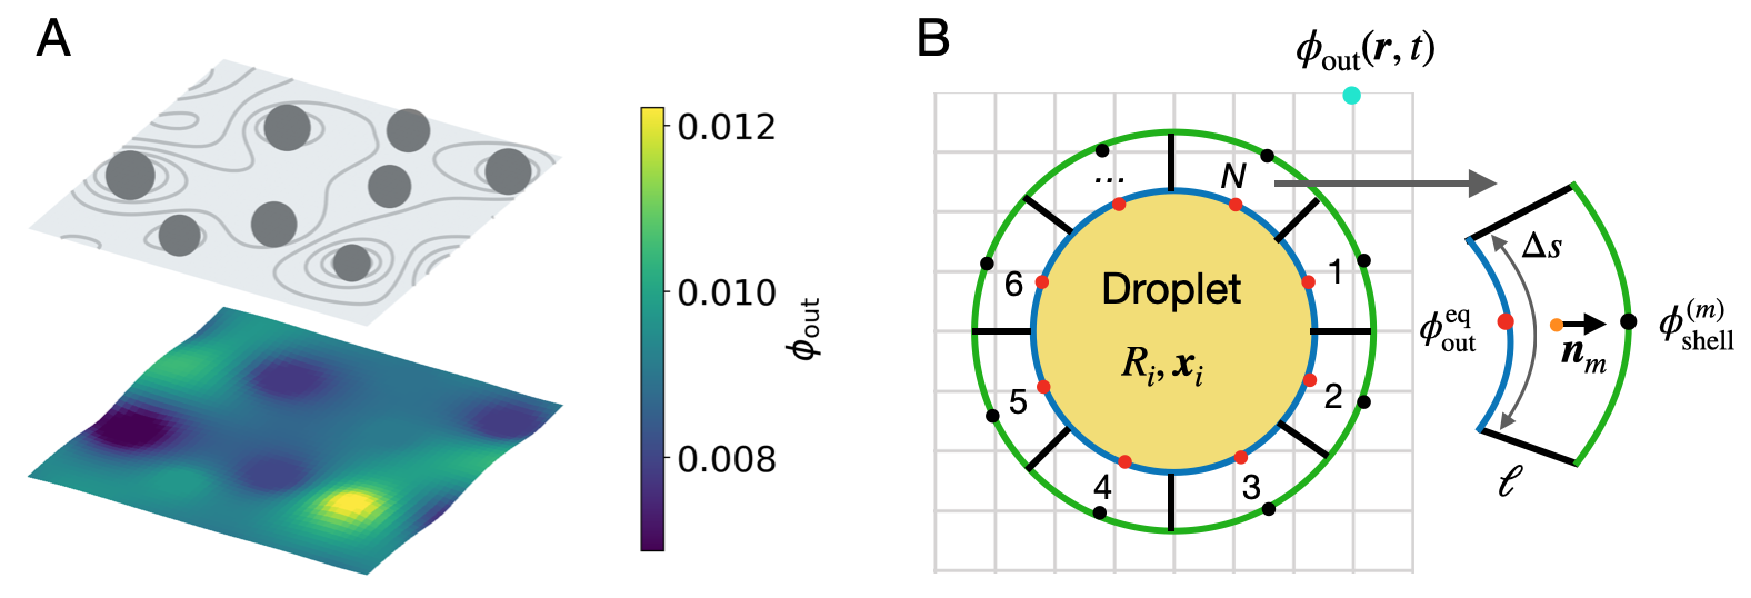
\includegraphics[scale=0.53]{MainContent/Figures/simulation.pdf}
\caption{\textbf{Schematics of the simulation model, describing droplets and the background field $\phiOut$.}
(A) Droplets (top plane, gray spheres) co-exist with the background field $\phiOut$ (bottom plane) and interact with it only through material fluxes.
For simplicity, $\phiOut$ also exists at the location of the droplets, but this has negligible effect on the dynamics.
Gray lines (top plane) show lines of similar background field $\phiOut$.
Dense lines indicate higher $\phiEqOut$ for smaller droplets.
(B) Isolated droplet (yellow) with a surrounding shell of thickness $\ell$ (green), which is further discretized in $N$ sectors of linear size $\ds$.
The exchanged fluxes between droplet and background are determined in each sector based on the equilibrium fraction $\phiEqOut$ (red dots) and the value $\phiOut^{(m)}$ at the outer side (black dot), which is determined from the background field using linear interpolation.
The background field $\phiOut$ is uniformly discretized on a Cartesian grid (cyan dots, gray grid).
}
\label{fig:schematics}
\end{figure}


\subsection{Dynamics of the background field}

Generally, the dynamics of the background field $\phiOut$ is affected due to diffusion and reactions, even if droplets are absent.
Additionally, if the droplets are present, material fluxes might flow in or out of the background field, eventually affecting the dynamics of $\phiOut$.
To numerically capture the dynamics of $\phiOut$, we discretize the continuous field $\phiOut$ on a uniform Cartesian grid with a spatial discretization $\dx$ between the neighbouring support points.
We then evolve \Eqref{eqn:RD_dilute} for a given chemical reaction scheme $s(\phiOut)$ in time using finite differences and an explicit temporal stepping, using a simulation package \textit{py-pde}, written in \textit{Python} and developed in the Zwicker Group; see Ref. \cite{Zwicker2020}.

Note that since we do not need to resolve droplets at this scale, the spatial discretization $\dx$ can be much larger than the interface width $w$, enabling us to simulate the background field using \Eqref{eqn:RD_dilute} at significantly lower computational costs (and higher speeds) compared to the continuous model \Eqref{eqn:CHActive}.
We next discuss the extent to which a single droplet alters $\phiOut$ in it's vicinity, enabling us to approximately calculate $\jOut$ outside the droplet. 

\subsection{Single droplet in an anisotropic environment}

To obtain the fluxes in the outer vicinity of an isolated droplet, we need to determine $\phiOut$ in the region surrounding this droplet.
In general the vicinity of the droplet might be anisotropic.
We discretize the heterogeneous vicinity of the droplet by constructing an annular region of thickness $\ell$ surrounding the droplet.
We further discretize this shell into $N$ annular shell sectors; see Fig. \ref{fig:schematics}B, to resolve spatial anisotropies of $\phiOut$ near the droplet.
These sectors are chosen uniformly in the angular directions for 2 and 3 dimensions and we assume that $N$ is large so that fluxes in the angular directions are negligible.

We then denote the volume fraction of the droplet material in the $m$-th sector as $\phiOut^{(m)}(r)$, where $r$ is a radial coordinate measuring the distance of the droplet surface from the droplet position $\vec{x}$.
Assuming that the dynamics of $\phiOut^{(m)}(r)$ in the shell sector relaxes quickly relative to the droplet growth and drift, we can determine $\phiOut^{(m)}(r)$ using \Eqref{eqn:RD_dilute} in stationary state along with the boundary conditions $\phiOut^{(m)}(R)=\phiEqOut$ and $\phiOut^{(m)}(R + \ell)= \phiShell^{(m)}$.
Here, $\phiShell^{(m)}$ is the fraction of droplet material in the background field at the outer side of the $m$-th shell sector, which we estimate from a linear interpolation of the discretized background field $\phiOut$; see Fig. \ref{fig:schematics}B.
Thus $\phiShell^{(m)}$ is an approximate representative volume fraction of the background field at the outer surface of the shell. 
Solving \Eqref{eqn:RD_dilute} would require information about the reaction flux $s(\phiOut)$ inside the shell sector, which we will discuss next.

Next, we focus our attention on the reaction flux inside the sector, given by $s(\phiOut^{(m)})$ from \Eqref{eqn:RD_dilute}, and determine it's effect on the dynamics of $\phiOut^{(m)}(r)$ inside the $m$-th shell sector.
We assume that $\phiOut^{(m)}(r)$ varies only marginally in the shell sector which allows us to linearize the reaction flux as a function of $\phiOut^{(m)}$ as:
\begin{equation*}
    s(\phiOut^{(m)}) \approx \Gamma_\mathrm{out} - \kOut~\phiOut^{(m)},
\end{equation*}
where
\begin{subequations} 
\label{eqn:GammaOut_KOut}
\begin{align}
    \Gamma_\mathrm{out} &= \frac{\phiShell^{(m)}~s(\phiEqOut) - \phiEqOut~s(\phiShell^{(m)})}{\phiShell^{(m)} - \phiEqOut} 
    \qquad \text{and}
    \\[10pt]
    \kOut &= \frac{s(\phiEqOut) - s(\phiShell^{(m)})}{ \phiShell^{(m)} - \phiEqOut},
\end{align}
\end{subequations}
are obtained from the boundary constraints $s(\phiOut^{(m)})(R) = s(\phiEqOut)$ and $s(\phiOut^{(m)})(R + \ell) = s(\phiShell^{(m)})$.
Taken together, the dynamics of $\phiOut^{(m)}(r)$ inside the shell sector can finally be determined from the steady state of \Eqref{eqn:RD_dilute} as:

\begin{equation}
\label{eqn:phi_out_in_shell}
     D_\mathrm{out}  \nabla ^2 \phiOut^{(m)}(r) + \Gamma_\mathrm{out} - \kOut~\phiOut^{(m)}(r) \approx 0,
\end{equation}
which can be analytically solved for $\phiOut^{(m)}(r)$; see Appendix \ref{sec:fluxes_inside_shell}.
Note that here we implicitly assume that the angular discretization of the shell is small enough, so that $\phiOut^{(m)}$ is only a function of the radial co-ordinate, which is the case for a large $N$.

Solving for $\phiOut^{(m)}$ gives us the local material fluxes outside the droplet surface for each sector in the normal direction as $\jOut^{(m)} \cdot \vec{n} = [-D_\mathrm{out} {\boldsymbol{\nabla}} \phiOut^{(m)}(R)] \cdot \vec{n} $, where $D_\mathrm{out}$ is the diffusivity outside the droplet.
We thus arrive at the fluxes outside the droplet; see Appendix \ref{sec:fluxes_inside_shell}.
Knowing the flux $\jOut^{(m)} \cdot \vec{n}$ outside each droplet for each $m$-th shell sector, we next determine the growth and drift of a system of droplets.

\subsection{Growth and drift of a system of droplets}

To briefly summarize, we obtain an analytical approximation of $\phiOut^{(m)}(r)$ in each shell sector, from which we determine the local flux $\jOut^{(m)}$ for a shell sector of a single isolated droplet.
We now consider a system of droplets much bigger than the interface width ($R \gg w)$ and neglecting the small value of $\phiEqOut$, the interfacial velocity then reads from \Eqref{eqn:InterfacialSpeed} as:
\begin{equation*}
    % \label{eqn:InterfacialSpeed_simplified}
    v_\mathrm{n} \approx \frac{\jIn - \jOut}{\phiEqIn} \cdot \vec{n},
\end{equation*}
Using the expression for $\jIn$ from \Eqref{eqn:flux_inside} along with the expression for $\jOut^{(m)} \cdot \vec{n}$ for the $m$-th shell sector; see Appendix \ref{sec:fluxes_inside_shell}, we finally arrive at a discretized form of \Eqsref{eqn:droplet_dynamics} for each droplet as:

\begin{subequations} 
\label{eqn:DropletDiscretized}
\begin{align}
    \frac{\Delta R}{\Delta t} &\approx \frac{1}{\phiEqIn}~\sum_{m=1}^{N} \frac{A_m}{S}\left ( \frac{R}{d}~s(\phi^\mathrm{eq}_\mathrm{in})  -  {j}^{(m)}_\mathrm{out}  \right)
    \mathrm{~and~}
    \\[10pt]
    \frac{\Delta \vec{x}}{\Delta t} &\approx \frac{d}{\phiEqIn}~\sum_{m=1}^{N} \frac{A_m}{S} \left ( \frac{R}{d}s(\phi^\mathrm{eq}_\mathrm{in})  -  {j}^{(m)}_\mathrm{out}\right) \vec{n}_m,
\end{align}
\end{subequations}
where $R, S, V$ are the radius, surface area and volume of the droplet respectively, $d$ is the space dimension, $A_m$ is the inner area of the shell sector, $d$ is the space dimension and $\vec{n}_m$ is the unit vector pointing from the droplet center to the $m$-th shell center; (orange dot, see \figref{fig:schematics}B).
\Eqsref{eqn:DropletDiscretized} can then be easily extended to encompass the description of multiple droplets and we thus arrive at the set of dynamical equations for describing growth and drift of a system of droplets.
Note that for the droplets to drift, the fluxes $\jOut^{(m)}$ necessarily need to be anisotropic with respect to the droplet.
This can be easily seen from the fact that if the droplet vicinity is isotropic, the droplet will simply grow and not drift. 

We thus use \Eqsref{eqn:DropletDiscretized} to describe how internal reactions and external material exchange with the background field affects the dynamics of each droplet.

\subsection{Coupling of droplets and background field}

We next describe a crucial part of the numerical scheme which involves coupling of the droplets with the background field. 
\Eqsref{eqn:DropletDiscretized} describes how droplets change when they take up droplet material from the background field $\phiOut$.
Recall that the local flux $\jOut^{(m)} \cdot \vec{n}$ enters the shell sector at the inner shell sector boundary (red points in \figref{fig:schematics}B).
Due to material conservation, the integrated flux $\Sigma = \jOut^{(m)} \cdot \vec{n}\,A_m$ needs to be removed from the background field $\phiOut$ for each shell sector of each droplet at the midpoint of the inner shell sector boundary (red points in \figref{fig:schematics}B).
Similar to the procedure when estimating $\phiShell^{(m)}$ from $\phiOut$, we again use a linear interpolation to remove the respective amount from the background field $\phiOut$.
Note that negative fluxes $\jOut^{(m)}$ distribute material from the droplets to the background field.
This procedure ensures that the total material flux toward the droplet is taken from the background field and it preserves potential anisotropies of the exchange.

\subsection{Choosing the time-step $\dt$}

We discuss the procedure for calculating the time-step $\dt$ used in the numerical model, which is a crucial simulation parameter as it potentially affects droplet growth and drift; see \Eqsref{eqn:DropletDiscretized}, as well as the dynamics of the background field $\phiOut$; see \Eqref{eqn:RD_dilute}.
Naturally, we wish to select a maximum allowed time-step which accurately captures the dynamics of the droplets and the background field. 

Hence, $\dt$ should be chosen based on the minimum of the time-steps involved when evolving:
\begin{enumerate}
    \item The dilute field $\phi_{\mathrm{out}}$ in time, according to \Eqref{eqn:RD_dilute}.
    
    \item The dynamics of the background $\phiShell^{(m)}(r)$ inside the $m$-th shell sector, as described by \Eqref{eqn:phi_out_in_shell}.
    
    \item The dynamics of the droplets in time, according to \Eqsref{eqn:DropletDiscretized}.
    
    \item The time-step arising from chemical reactions.
\end{enumerate}
Naturally, smaller values of $\dt$ imply more accurate simulations and larger values result in faster (but less accurate) simulations.
% ; although very low or very high time-steps numerical instabilities might also render the simulations unstable.
% These instabilities can potentially arise from choosing a small shell thickness $\ell$, which results in a large value of fluxes outside the droplet $\jOut^{(m)} \cdot \vec{n}$, as they scale with $\ell^{-1}$; see Appendix \ref{sec:fluxes_inside_shell}.
% Another potential area of origin for instabilities is when $\ds$ is a small quantity, which 
We next separately analyze the dynamics of the background field, the shell, and the droplet growth to identify the maximal suitable value of $\dt$.

In general, the time-step for evolving \Eqref{eqn:RD_dilute} is determined from the mutual interplay between reactions and diffusion.
A standard von Neumann stability analysis of \Eqref{eqn:RD_dilute} shows that our numerical scheme is stable if $\dt < \dx^2/(2 D_\mathrm{out})$, where $D_\mathrm{out}$ is the diffusivity outside the droplet.
Consequently, a suitable time-step for evolving the background field is $\dt_\mathrm{background} = 0.1 \dx^2/D_\mathrm{out}$, where we choose the constant pre-factor conservatively as $0.1$ instead of $0.5$.
Similarly, we define $\dt_\mathrm{shell} = 0.1 \ell^2/D_\mathrm{out}$ for the shell.
We also consider the time scale of reactions, $\dt_\mathrm{reaction} = 0.1 / (\max_\phi |s(\phi)|)$, based on the maximal rate of $s(\phiOut)$ to accurately capture the effect of chemical reactions on the dynamics of $\phiOut$.

Finally, to ensure that the dynamics of droplet growth is captured correctly, we assume the droplet growth rate ($\Delta R / \Delta t$) at each time-step to be proportional to their radius $R$ (neglecting the $1/R^2$ dependence); see Ref. \cite{Review2019}, and limit the droplet growth rate from \Eqsref{eqn:DropletDiscretized} to $10\%$ of their previous size.
In other words, we place a restriction such that the relative growth of a single droplet $R^{-1}\abs{\diff R/\diff t}$ is small during a single time-step $\dt$.
Assuming that typical droplets are not much smaller than the mean initial droplet radius~$\mean{R}$, this implies a maximal time-step $\dt_\mathrm{droplets} = 0.1 \mean{R}^2/D_\mathrm{out}$.
This is specially important when considering mean-field simulations as time-step $\dt$ would be too high if it is calculated solely on the basis of the shell thickness $(\dt_\mathrm{shell})$ and the background field discretization $(\dt_\mathrm{background})$.
Such a large time-step will erroneously calculate the droplet dynamics from \Eqsref{eqn:DropletDiscretized} and hence we have to consider the size of the droplets as well when calculating the time-step $\dt$.
Finally, we choose the time-step $\dt$ which is a conservative minimum of all the different time-steps mentioned above, i.e.
\begin{equation}
\label{eqn:time_step}
    \dt = 0.1 \, \mathrm{min \, }\left[  \frac{0.1 \dx^2}{D_\mathrm{out}}, \frac{0.1 \mean{R}^2}{D_\mathrm{out}}, \frac{0.1 \ell^2}{D_\mathrm{out}}, \frac{0.1}{(\max_\phi |s(\phi)|)} \right ].
\end{equation}

\subsection{Algorithm and full simulation}

The full numerical method involves evolving the state of the system, i.e., the discretized background field $\phiOut(\vec{r})$ and the positions $\vec{x}_i$ and radii $R_i$ of all droplets in time.
We perform an explicit iteration in time, where the state at $t + \dt$ is directly determined from the state at time $t$.
We first evolve the reaction-diffusion equation \Eqref{eqn:RD_dilute} of the background field and then iterate over all droplets.
For each droplet, we determine the fluxes $\jOut^{(m)} \cdot \vec{n}$ outside the $m$-th sector. We then remove the associated material from the background field for all $N$ shell sectors and update the droplet's position and radius according to \Eqsref{eqn:DropletDiscretized}.
Starting from an initial state at $t=0$, the numerical algorithm (see Algorithm \ref{alg:algorithm}), allows us to evolve the dynamics forward in time.

\section{Summary}

As we were interested primarily in simulating dynamics of phase separated droplets and background field, we built upon the thin-interface approximation model given by \Eqsref{eqn:thin_interface_model} from Chapter \ref{chap:Chapter_2}, which separately describes the dynamics of droplets and the background field.
This model is an approximation of the continuous model given by \Eqref{eqn:CHActive}.
To accurately model the dynamics of the droplets, we needed to calculate the material fluxes in the droplets $\jIn$ and outside the droplets $\jOut$, which govern how much material enters or exits the droplets, thus affecting their dynamics.

We first described the dynamical equations for the volume fraction inside the droplet $\phiIn$ from \Eqref{eqn:RD_droplet} and calculated $\jIn$ from \Eqref{eqn:flux_inside} based on chemical weak reactions.
Assuming that we knew the volume fraction outside the droplets $\phiOut$ in principle from \Eqref{eqn:RD_dilute}, $\jOut$ outside the droplet could then be evaluated, leading to the interfacial speed $\vn$ from \Eqref{eqn:InterfacialSpeed}, which led us to formulating the dynamical equations of growth and drift for spherical droplets given by \Eqsref{eqn:droplet_dynamics}.

We then focused on calculating the fluxes outside the droplets $\jOut$, which stem from spatial gradients in $\phiOut$.
In principle, dynamics of $\phiOut$ followed from the dynamical equation \Eqref{eqn:RD_dilute} with appropriate boundary conditions at the droplet surfaces.
However, we greatly simplified the description of $\phiOut$ by assuming that $\phiOut$ also exists at locations where the droplets exist as well; see \figref{fig:schematics}A, and that the $\phiOut$ is slightly altered near the droplets in the presence of the droplets. 
This meant that the dynamical equation for $\phiOut$ \Eqref{eqn:RD_dilute} no longer needed complicated boundary conditions at the locations of the droplets, but only boundary conditions at the edges of the domain. 

Since droplets altered the background field near them, we wanted to quantify this influence in order to accurately calculate the fluxes outside the droplet.
To that end, we discretized the surroundings of each droplet by considering annular shell sectors of thickness $\ell$ and angular width $\ds$.
To obtain the fluxes in the $m$-th shell sector $\jOut^{(m)}$, we needed the volume fraction field outside the droplet $\phiOut^{(m)}$, which we solved from \Eqref{eqn:phi_out_in_shell}.
The boundary conditions used to solve \Eqref{eqn:phi_out_in_shell} were $\phiOut^{(m)}(R)=\phiEqOut$ and $\phiOut^{(m)}(R + \ell)= \phiShell^{(m)}$ and $\phiShell^{(m)}$ was approximated from a linear interpolation of the background field $\phiOut$.
We thus arrived at the fluxes outside the droplet, enabling us to write the numerical counterpart of \Eqsref{eqn:droplet_dynamics} as \Eqsref{eqn:DropletDiscretized}.

We then determined the coupling between the background field and the droplets by removing the same amount of material from the background field that enters the droplets, hence conserving mass.
Next, we discussed the time-step $\dt$ calculations by considering four different time-steps based on von Neumann stability analysis of \Eqref{eqn:RD_dilute}, and considering the minimum of them as the final time-step $\dt$ from \Eqref{eqn:time_step}.
Finally, we formulated the numerical algorithm; see Algorithm \ref{alg:algorithm}, for evolving droplet dynamics from \Eqsref{eqn:DropletDiscretized} and background field $\phiOut$ from \Eqref{eqn:RD_dilute}, using the time-step $\dt$ from \Eqref{eqn:time_step}.

\newpage

\begin{algorithm}

\label{alg:algorithm}

$\bullet$ Input values for model parameters: $b, \kappa, \Lambda, \phi^{(0)}_\mathrm{in}, \phi^{(0)}_\mathrm{out}$\;

$\bullet$ Input initial radii $(R_i)$ and position $(\vec{x}_i)$ of all droplets\;

$\bullet$ Calculate diffusivity outside the droplets $D_\mathrm{out} = \Lambda(\phi^0_\mathrm{out}) \, b$\;

$\bullet$ Input initial volume fraction of the dilute field $\phiOut(\vec{r}, t=0)$\;

$\bullet$ Input formulation for chemical reaction fluxes $s(\phiIn),~s(\phiOut)$ inside and outside the droplet respectively\;

$\bullet$ Define total simulation time $T_\mathrm{max}$\;

$\bullet$ Set values for simulation parameters $\dx, \ell, \ds$\;

\SetKwProg{Pn}{Function}{:}{\KwRet}
\Pn{\FMain{$\left \langle R_i  \right \rangle, \ell, \Delta x, s(\phiOut), D_\mathrm{out}$}}
{
    $\bullet$ Estimate time-step $\Delta t$ for the simulation from \Eqref{eqn:time_step}\;
}
% \For{($t < T_{max}$)}{
\While{$(t < T_\mathrm{max})$}{
    \For{($\mathrm{single~droplet~of~radius~}R$)}
    {
        $\bullet$ Calculate capillary lengths $l_{\gamma, \mathrm{out}}, l_{\gamma, \mathrm{in}}$ from \Eqref{eqn:l_gamma}\;
        
        \SetKwProg{Pn}{Function}{:}{\KwRet}
        \Pn{\FMain{$R, l_{\gamma, \mathrm{out}}, l_{\gamma, \mathrm{in}}, \phi^\mathrm{0}_\mathrm{out}, \phi^\mathrm{0}_\mathrm{in}$}}
        {
            $\bullet$ Calculate equilibrium volume fractions $\phiEqIn, \phiEqOut$ from \Eqref{eqn:GibbsThompsonRelations}\;
        }
        
        $\bullet$ Construct the annular shell of thickness $\ell$ around the droplet\;
        
        $\bullet$ Discretize the droplet surface into $N$ uniformly spaced shell sectors and locate the co-ordinates of their midpoints (in black; see Fig. \ref{fig:schematics}B)\;
        
        \For{(the $m^{\mathrm{th}}$ shell sector out of $N$ sectors)}{
        
            $\bullet$ Calculate $\phiShell^{(m)}$ (in black; see Fig. \ref{fig:schematics}B) from linear interpolation of grid-points of $\phiOut$ (in cyan, see Fig. \ref{fig:schematics}B)\;
            \SetKwProg{Pn}{Function}{:}{\KwRet}
            \Pn{\FMain{$\phiShell^{(m)}, \phiEqOut, s(\phiEqOut), s(\phiShell^{(m)})$}}
            {
                $\bullet$ Evaluate $\Gamma_\mathrm{out}, k_\mathrm{out}$ from \Eqsref{eqn:GammaOut_KOut}\;
            }
            \SetKwProg{Pn}{Function}{:}{\KwRet}
            \Pn{\FMain{$\phiEqIn, \phiEqOut, \phiShell^{(m)}, D_\mathrm{out}, R_i, \Gamma_\mathrm{out}, k_\mathrm{out}, \ell$}}
            {
                $\bullet$ Calculate volume fraction inside the shell sector $\phiOut^{(m)}(r)$ from \Eqref{eqn:phi_out_in_shell} with boundary conditions $\phiOut^{(m)}(R) = \phiEqOut$ and $\phiOut^{(m)}(R + \ell) = \phiShell^{(m)}$\;
                
                $\bullet$ Evaluate fluxes outside the droplet $\jOut \cdot \vec{n}$ from $\phiOut^{(m)}(r)$; see Appendix \ref{sec:fluxes_inside_shell}\;
            }

            $\bullet$ Locate the co-ordinates of points of material exchange (in red; see Fig. \ref{fig:schematics}B)\;

        	$\bullet$ Remove amount equal to $\jOut^{(m)} \cdot \vec{n}\,A_m$ from the background field $\phiOut$, at the points of material exchange\;
        
        }

        $\bullet$ Calculate total amount of fluxes outside the droplet by summing up the contributions of $\jOut$ from all $N$ shell sectors\;

        $\bullet$ Calculate total amount of fluxes inside the droplet $\jIn$ from \Eqref{eqn:flux_inside}\;

        $\bullet$ Update the droplet radii and position using \Eqsref{eqn:DropletDiscretized}\;
    }

    $\bullet$ Evolve $\phiOut$ from \Eqref{eqn:RD_dilute} using time-step $\dt$ on the entire domain\;

    $\bullet$ Obtain updated $\phiOut$ and updated position and radii for all droplets at time $t + \dt$\;
}
\rule{\textwidth}{0.5pt}
\caption{
Numerical algorithm for evolving droplet dynamics from \Eqsref{eqn:DropletDiscretized} and background field $\phiOut$ from \Eqref{eqn:RD_dilute}.
}
\end{algorithm}

